\chapter{Numerical treatment}
\label{chap:num}
% * numerical treatments necessary
% * main goal: calculate reduced density operator
% * other things: absorption spectra, single trajectories


%%%%%%%%%%%%%%%%%%%%%%%%%%%%%%%%%%%%%%%%%%%%%%%%%%%%%%%%%%%%%%%%%%%%%%%%%%%%%%%
\section{Hierarchical Equations of Motion}
\label{sec:num.heom}
% * Tanimura HEOMs
%%%%%%%%%%%%%%%%%%%%%%%%%%%%%%%%%%%%%%%%%%%%%%%%%%%%%%%%%%%%%%%%%%%%%%%%%%%%%%%


%%%%%%%%%%%%%%%%%%%%%%%%%%%%%%%%%%%%%%%%%%%%%%%%%%%%%%%%%%%%%%%%%%%%%%%%%%%%%%%
\section{Stochastic Hierarchical Equations of Motion}
\label{sec:num.sheom}
% * main idea
%
% TODO more general cases?
%%%%%%%%%%%%%%%%%%%%%%%%%%%%%%%%%%%%%%%%%%%%%%%%%%%%%%%%%%%%%%%%%%%%%%%%%%%%%%%

In this section we present one of the main results of this work, namely a numerical method to solve the non-Markovian stochastic Schrödinger equation
\begin{equation}
  \partial \psi_t = -\ii h \psi_t + L\ZZ_t \psi_t - \adj{L}\int_0^t \alpha(t-s) \frac{\delta\psi_t}{\delta\ZZ_s} \dd s
  \label{eq:num.nmsse}
\end{equation}
without making use of the $O$-operator substitution.
Therefore we need to conceive a different way to deal with the nonlocality of the functional derivative with respect to time and the noise-process, as it prevents us from employing the common techniques for dealing with stochastic Schrödinger equations in the Markovian regime \cite{???}.

It turns out that for certain correlation functions the linear NMSSE~\ref{eq:num.nmsse} is formally equivalent to an infinite hierarchy of completely local stochastic differential equations.
% TODO Really?
Although we borrow the main idea from the hierarchical equations of motion presented in the last section, we need to deal with some peculiarities of our NMSSE first.

%%%%%%%%%%%%%%%%%%%%%%%%%%%%%%%%%%%%%%%%%%%%%%%%%%%%%%%%%%%%%%%%%%%%%%%%%%%%%%%
\subsection{Time derivation}
%TODO change title
\label{sub:num.sheom.time_deriv}

% TODO Make clear, that we dont imply normalization
The basic idea is to absorb the action of the functional derivative on $\psitZ$ into an auxiliary stochastic pure state
\begin{equation}
  \psitZ[1] := \int_0^t \alpha(t - s) \frac{\delta \psi_t(\ZZ)}{\delta \ZZ_s} \dd s.
  \label{eq:num.first_order}
\end{equation}
We recall that the integral boundaries arise only after we apply the derivative on states $\psi_t(\ZZ)$ that satisfy the additional condition $\delta \psitZ / \delta \ZZ_s = 0$ for $ s < 0$ and $s > t$.
Therefore we may write \autoref{eq:num.first_order} more concise as
\begin{equation*}
  \psitZ[1] = \left( \int \alpha(t - s) \frac{\delta}{\delta \ZZ_s} \dd s \right) \psitZ =: \adjZZ_t \psitZ
\end{equation*}
with the integrated functional derivation operator $\adjZZ_t$.

% TODO Hierarchies for arbitrary α?
The first step toward deriving an equation of motion for $\psitZ[1]$ is answering the question under which conditions a simple expression for $\dot\adjZZ_t$ exists.
Since the latter is given by $\dot\adjZZ_t = \int\dot\alpha(t-s) \, \delta / \delta \ZZ_s \dd s$ we assume an exponential bath correlation function
\begin{equation}
  \alpha(t) = g \, \exp[-\gamma \abs{t} - \ii \Omega t] = g \exp[-\ii \Omega t] \left( \Theta(t) \exp[-\gamma t] + \Theta(-t) \exp[\gamma t] \right).
  \label{eq:num.exp_bcf}
\end{equation}
with the Heaviside function $\Theta$.
As the singular terms in the time derivative cancel we obtain
\begin{equation*}
  \dot\alpha(t) = g \exp[-\ii \Omega t] \left( (-\gamma - \ii\Omega) \Theta(t) \exp[-\gamma t] + (\gamma - \ii\Omega)\Theta(-t)\exp[\gamma t] \right).
\end{equation*}
Therefore we cannot exploit $\dot\adjZZ_t \propto \adjZZ_t$ on the level of operators in general.
Even the vanishing of the functional derivative $\delta \phi_t(\ZZ) / \delta \ZZ_s$ for $s > t$ with some arbitrary stochastic state $\phi_t(\ZZ)$ does not imply $\dot\adjZZ_t \phi_t(\ZZ) \propto \adjZZ_t\phi_t(\ZZ)$ as the following example shows:
Take $\phi_t(\ZZ) = \varphi \cdot (\ZZ_t + \ZZ_{t'})$ for some noise independent system state $\varphi$ and $0 < t' < t$.
It clearly satisfies the required boundary conditions, but
\begin{equation*}
  \dot\adjZZ_t \phi_t(\ZZ) = (\dot\alpha(0) + \dot\alpha(t-t')) \varphi = \left( -2\ii\Omega - (\gamma + \ii\Omega) \exp[-(\gamma + \ii\Omega) (t-t')] \right) \varphi
\end{equation*}
which is not proportional to
\begin{equation*}
  \adjZZ_t \phi_t(\ZZ) = (\alpha(0) + \alpha(t - t')) \varphi = g (1 + \exp(-\gamma + \ii \Omega)(t-t')) \varphi.
\end{equation*}
We see that the problematic first summand arises due to singular behavior of $\delta \phi_t(\ZZ) / \delta \ZZ_s$ for $s = t$.

% TODO Where.
Such problems do not occur once we restrict $\dot\adjZZ_t$ to solutions of our NMSSE~\ref{eq:num.nmsse} with vacuum initial conditions.
Indeed we see from \autoref{eq:???} that the functional derivative of $\psitZ$ at the upper boundary is regular and therefore has vanishing weight under the integral.
Hence we obtain for the time derivative of our integrated derivation operator
\begin{equation}
  % TODO Watch for change in \psitZ
  \dot\adjZZ_t \psitZ = - (\gamma + \ii \Omega) \adjZZ_t\psitZ
  \label{eq:num.dot_adjZZt}
\end{equation}
In the remaining work we use the shorthand notation $w = \gamma + \ii\Omega$.
% TODO Finalize!

%%%%%%%%%%%%%%%%%%%%%%%%%%%%%%%%%%%%%%%%%%%%%%%%%%%%%%%%%%%%%%%%%%%%%%%%%%%%%%%
\subsection{Linear Hierarchy}
\label{sub:num.sheom.lin}
% * derivation
% * terminator
%
% TODO Surpession by γ / Ω; differences, in the following combined into w
% TODO Time-local/nonlocal terminators

We now return to our non-Markovian stochastic Schrödinger equation; with the auxiliary stochastic state~\ref{eq:num.first_order} it can written as
\begin{equation*}
  \partial_t \psitZ = -\ii\Hsys\psitZ + L\ZZ_t\psitZ - \adj{L}\psitZ[1].
\end{equation*}
Hence if we can derive a tractable equation of motion for $\psitZ[1]$ we reduce the problems with a functional derivative to propagating a coupled system of simpler equations.
With the result from the last section \autoref{eq:num.dot_adjZZt} and the original NMSSE~\ref{eq:num.nmsse} we find
\begin{align}
  \partial_t (\adjZZ_t \psi_t) &= - w \adjZZ_t\psi_t + \adjZZ_t ( -\ii\Hsys + L\ZZ_t - \adj{L} \adjZZ_t ) \psi_t \nonumber \\
  &= (-\ii\Hsys - w + L\ZZ_t) \psit[1] + [\adjZZ_t, \ZZ_t] L\psit - \adj{L} \adjZZ_t \psit[1],
  \label{eq:num.dot_psi1}
\end{align}
where we use that $\adjZZ_t$ commutes with all system operators.
It is not surprising that the functional derivative reappears in the equation for $\psit[1]$; therefore we need to introduce another auxiliary state.
This scheme leads to an infinite hierarchy of auxiliary states defined by
\begin{equation}
  \psit[k] := \adjZZ_t \psit[k-1] = \adjZZ_t^k \psit.
  \label{eq:num.auxiliary_states}
\end{equation}
Expressed in the new auxiliary states and with $[\adjZZ_t, \ZZ_s] = \alpha(t-s)$ \autoref{eq:num.dot_psi1} reads
\begin{equation*}
  \partial_t \psit[1] = (-\ii\Hsys - w + L\ZZ_t) \psit[1] + \alpha(0) L\psit[0] - \adj{L}\psit[2].
\end{equation*}
Along these lines it is straightforward to derive the full hierarchy of equations of motions for all $\psit[k]$.
Since the commutator $[\adjZZ_t, \ZZ_s]$ is a $\Complex$-number each auxiliary state only couples to the order directly above and below
% TODO More steps?
\begin{equation}
  \partial_t\psit[k] = (-\ii\Hsys - kw + L\ZZ_t)\psit[k] + k \alpha(0) \psit[k-1] - \adj{L} \psit[k+1].
  \label{eq:num.hierarchy_lin}
\end{equation}
The vacuum initial condition for the true quantum trajectory $\delta \psi_0 / \delta \ZZ_s = 0$ requires that all auxiliary states vanish at $t=0$.

% TODO Check grammar
Of course the infinite hierarchy is even more intricate to solve than the original non-Markovian stochastic Schrödinger equation; therefore we need to truncate at some finite order.
It is quite remarkable that this can be done in a self-consistent manner, which even approximately incorporates all truncated orders into the remaining equations.
We start by transforming \autoref{eq:num.linear_hierarchy} into an equivalent integral equation.
Notice that
\begin{align}
  \psit[k + 1] = &\int_0^t \exp[-(k+1)w(t-s)] \Texp[\int_s^t -\ii\Hsys + L\ZZ_u \dd u] \nonumber \\
  &\left( (k+1) \alpha(0)L\psi_s^{(k)} - \adj{L} \psi_s^{(k+2)} \right) \dd s
  \label{eq:num.terminator_integral}
\end{align}
% TODO "Formally" correct here?
formally satisfies the corresponding equation of motion together with the required initial condition.

% TODO Continue!

%%%%%%%%%%%%%%%%%%%%%%%%%%%%%%%%%%%%%%%%%%%%%%%%%%%%%%%%%%%%%%%%%%%%%%%%%%%%%%%
\subsection{Nonlinear Hierarchy}
\label{sub:num.sheom.nonlin}
% * derivation

We mention in \autoref{sec:nmqsd.nonlin_nmsse} how the scaling of our Monte-Carlo sampling with the number of realizations improves drastically we use a nonlinear version.
This can be achieved within our microscopical using the comoving coherent states defined in \autoref{eq:nmqsd.comoving_flow}.
Up to a certain extend this method can also be employed for our hierarchical equations of motion.

As a function of the coherent state labels $\cc\zz$ instead of the process $\ZZ$ we define comoving auxiliary states by
\begin{equation*}
  \tilde\psi_t^{(k)}(\cc\zz) := (\psit[k] \circ \vec\phi_t)(\cc\zz) = \psit[k](\vec\phi_t(\cc\zz)).
\end{equation*}
Then the same steps that give \autoref{eq:nmqsd.nmsse_nonlin} lead to a similar result
% TODO More steps?
\begin{align}
  \partial_t \tilde\psi_t^{(k)}(\cc\zz) &= \left( -\ii\Hsys - kw + L\ZZ_t + L \int_0^t \cc{\alpha(t-s)} \qmean{\adj L}_s \dd s \right)\tilde\psi_t^{(k)}(\cc\zz) \nonumber\\
  &+ k \alpha(0) L \tilde\psi_t^{(k-1)} - (\adj{L} - \qmean{\adj L}_t) \tilde\psi_t^{(k+1)}(\cc\zz),
  \label{eq:num.hierarchy_nonlin}
\end{align}
with the normalized expectation value taken with respect to the true quantum trajectory---or put differently with respect to the zeroth order auxiliary state
\begin{equation*}
  \qmean{\adj L}_s = \frac{\bra{\tilde\psi_t^{(0)}} \adj{L} \ket{\tilde\psi_t^{(0)}}}{\braket{\tilde\psi_t^{(0)}}{\tilde\psi_t^{(0)}}}.
\end{equation*}
Notice that the exponential correlation function necessary for the hierarchy also simplifies the treatment of the memory-term in \autoref{eq:num.hierarchy_nonlin}.
% TODO Improve!
Indeed we can derive a simple and closed evolution equation for it.

But one caveat remains: for the convolutionless formulation we can go one step further and even derive an equation for normalized pure state trajectories~\ref{eq:nmqsd.nmsse_nonlin_full}.
The same does not hold true for the hierarchical equations of motion.
% TODO Elaborate!

% TODO Terminator

%%%%%%%%%%%%%%%%%%%%%%%%%%%%%%%%%%%%%%%%%%%%%%%%%%%%%%%%%%%%%%%%%%%%%%%%%%%%%%%
\subsection{Multimodes}
\label{sub:num.sheom.nonlin}
% * rectangular vs triangular truncation
% TODO Change title
% TODO Seperate section in chapter 2?
% TODO Reference to Schulten paper?

Of course most physically interesting systems cannot be modeled with only a single exponential bath mode.
We now present the changes necessary to accommodate a more general environmental structure given by a finite number of exponential modes coupling to the system with arbitrary operators.
As the crucial points do not depend on the choice of linear or nonlinear version we are only concerned with the former in this section.

% TODO Grammar!
The linear non-Markovian stochastic Schrödinger equation for a finite number $N$ of independent environments may be derived along the same lines presented in \autoref{sec:nmqsd.lin_nmsse}.
It reads
\begin{equation*}
  \partial_t \psit = -\ii\Hsys\psit + \sum_{j=1}^N L_j \ZZ_{j, t} \psit - \sum_{j=1}^N \adj{L}_j \int_0^t \alpha_j(t - s) \frac{\delta \psit}{\delta \ZZ_{j, t}} \dd s
\end{equation*}
with independent noise processes satisfying
\begin{equation*}
  \E\,Z_{i, t} = 0, \quad \E\,Z_{i, t} Z_{j, s} =0, \quad\mbox{and}\quad \E\,Z_{i, t} \ZZ_{j, s} = \delta_{ij}\alpha_i(t-s).
\end{equation*}
Remember that our hierarchical equations of motion rely on an exponential bath correlation function; therefore we need to introduce several derivation operators $\adjZZ_{j, t}$, one for each process.
Just as in the single-mode case, the auxiliary states are obtained by successively applying $\adjZZ_{i, t}$ on the quantum trajectory $\psitZ$
\begin{equation}
  \psit[k_1, \dots, k_N] := \adjZZ_{1, t}^{k_1} \dots \adjZZ_{N, t}^{k_N} \psit.
  \label{eq:num.auxiliary_states_multi}
\end{equation}
Note that all $\adjZZ_{j, t}$ mutually commute.
Consequently \autoref{eq:num.auxiliary_states_multi} is the most general form how a functional derivative may occur in the derivation of the corresponding hierarchy.
Hereinafter we use the shorthand notation $\psit[\kk]$ for the auxiliary state defined above.
Similar to~\ref{eq:num.hierarchy_lin} its equation of motion reads
\begin{equation}
  \partial_t\psit[\kk] = (-\ii\Hsys - \kk\cdot\ww + \sum_j L_j \ZZ_{j, t})\psit[\kk] + \sum_j k_j \alpha_j(0) \psit[\kk - \ee_j] - \sum_j \adj{L}_j \psit[\kk + \ee_j],
  \label{eq:num.hierarchy_lin_multi}
\end{equation}
where $\ee_j$ denotes the $j$-th unit vector in $\Reals^N$ and $\kk\cdot\ww = \sum_j k_jw_j$ is the euclidean scalar product.\footnote{Although $\ww$ is complex in general no complex conjugation occurs at any time.}

% TODO Do this with pure tikz
\begin{figure}
  \centering
  \begin{subfigure}[b]{.4\columnwidth}
    \centering
    \includegraphics[scale=.85]{img/cubic_hierarchy}
    \caption{Quadratic}
    \label{fig:num.trunc_cubic}
  \end{subfigure}
  \begin{subfigure}[b]{.4\columnwidth}
    \centering
    \includegraphics[scale=.85]{img/triang_hierarchy}
    \caption{Triangular}
    \label{fig:num.trunc_tria}
  \end{subfigure}
  \caption{Comparison of the two truncation schemes in the special case of $N=2$ processes with order $D$.}
% TODO Insert more blabla
  \label{fig:num.trunc}
\end{figure}
% TODO Too much "states"
When it comes to truncating the hierarchy~\ref{eq:num.hierarchy_lin_multi} the most obvious strategy is simply to cut off each mode separately at given order $D$.
In other words the truncation condition reads $0 \le k_j \le D$ for all $j=1,\dots,N$; any auxiliary state not satisfying it is set to zero.
We refer to this scheme as \quotes{cubic truncation scheme} since the shape of all states under consideration resembles an $N$-cube (see also \autoref{fig:num.trunc_cubic}).
Clearly the number of auxiliary states scales exponentially like $(D+1)^N$, which makes the treatment of physically interesting systems with $N$ in the order of $100$ absolutely impossible.

Examining \autoref{eq:num.hierarchy_lin_multi} closer we notice that the term responsible for suppression of the $\kk$-th order auxiliary state is $\exp(-\kk \cdot \ww)$.
Instead of treating each mode individually we use a condition better suited for the product $\kk\cdot\ww$, namely $0 \le \abs{\kk} \le D$ with $\abs{\kk} = \sum_j k_j$.
For $N=2$ the corresponding states form a triangular shape as shown in \autoref{fig:num.trunc_tria}, hence the name \quotes{triangular truncation}.
The appropriate generalization to arbitrary $N$ is a simplex where the number of elements is given by
\begin{equation*}
  \sum_{d=0}^D {d + N - 1 \choose N - 1} \approx % TODO Stirling, Polynomial
\end{equation*}
showing a much softer scaling compared to the cubic scheme.
% TODO Polynomial for large N?
In \autoref{fig:num.scaling} we display the number of auxiliary states required for a given number of modes and truncation order $D$.
Clearly the triangular truncation is far superior although for small $N$ both methods are still feasible.
The difference is more pronounced for larger $N$ required in the study of realistic systems.
% TODO Done that? Really?
As an example take the Fenna-Matthews-Olson complex further investigated in \autoref{sec:num.fmo}:
In a simplified model we couple mutually independent environments with 13 exponential terms to each of its seven sites for a total of 91 modes.
This yields an insurmountable number of about $10^{30}$ auxiliary states for the cubic truncation in first order hierarchy, compared to only 5151 using the triangular scheme.

\begin{figure}
  \centering
  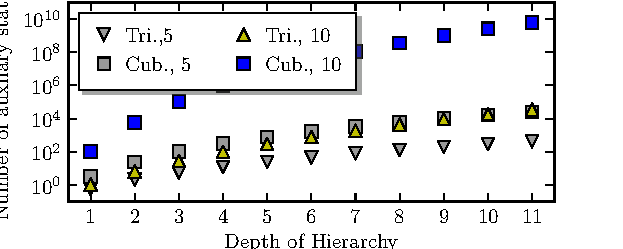
\includegraphics{img/scaling.pdf}
  \caption{Comparison\dots}
  \label{fig:num.scaling}
\end{figure}

% TODO Mention manual cutoff????

%%%%%%%%%%%%%%%%%%%%%%%%%%%%%%%%%%%%%%%%%%%%%%%%%%%%%%%%%%%%%%%%%%%%%%%%%%%%%%%
\section{Correlation Function Expansion}
\label{sec:num.expansion}
% * pade spectrum decomposition
% * also mention other (Matsubara e.g.)
% * uniqueness? Theoretically yes, in practices doesnt matter!
% * Plot for Ohmic spectral density (where do these appear?)
% * Show highly structured density, approximation!
%
% TODO Expansion of general spectral density; not unique!
%      Cool to use antisymmetric lorentzians
% TODO Discussion J(0) = 0 physical necessary, linear (ohmic) decrease, etc.

%%%%%%%%%%%%%%%%%%%%%%%%%%%%%%%%%%%%%%%%%%%%%%%%%%%%%%%%%%%%%%%%%%%%%%%%%%%%%%%

Applicability of our hierarchical equations of motion to any physically interesting system depends predominantly on the ability to express the relevant bath correlation function
\begin{equation}
  \alpha(t) = \int_0^\infty J(\omega) \left( \coth \frac{\beta \omega}{2} \cos \omega(t-s) - \ii\sin \omega(t-s) \right) \mathrm{d}s
  \label{eq:num.alpha_thermal}
\end{equation}
as a sum of exponentials like~\ref{eq:num.exp_bcf}.
Such exponential functions arise as Fourier transforms of a Lorentzian spectral density
\begin{equation}
  J(\omega) = \frac{1}{\pi} \frac{\gamma}{(\omega - \Omega)^2 + \gamma^2}.
  \label{eq:num.lorentzian}
\end{equation}
Hence they can be obtained from \autoref{eq:num.alpha_thermal} in the zero-temperature limit provided we extend the integral domain to include arbitrary negative frequencies as well.
% TODO Keep figure?
This unphysical assumption is a good approximation to the exact case without negative frequencies only for certain parameters as \autoref{fig:num.lorentzian} shows:
For $\gamma\ll\Omega$ the Lorentzian density $J$ is concentrated mostly on the positive semi-axis and the negative frequency contribution to \autoref{eq:num.alpha_thermal} can be neglected.
\begin{figure}
  \centering
  \includegraphics{img/lorentzian}
  \caption{Lorentzian spectral densities (see \autoref{eq:num.lorentzian} for notation).}
  % TODO More caption?
  \label{fig:num.lorentzian}
\end{figure}

A more systematic way to obtain the desired bath correlation function in the case $T > 0$ was proposed by Meier and Tannor \cite{MeTa99_non_markovian}.
They employ anti-symmetrized Lorentzian distributions $\tilde J(\omega) := J(\omega) - J(-\omega)$ to include the negative frequencies without any approximation.
% TODO "Indeed, since" good idea?; Check grammer in general!
Indeed, since $\tilde J$, $\coth$, and $\sin$ are anti-symmetric and $\cos$ is symmetric with respect to reflection at the origin we have
\begin{equation*}
  \int_0^\infty \tilde J(\omega) (\dots) \mathrm{d}\omega = \frac{1}{2}\int_{-\infty}^\infty \tilde J(\omega) (\dots) \mathrm{d}\omega.
\end{equation*}
Of course the same holds true for any anti-symmetric spectral density.
% TODO Mhhh...
However, the bath correlation function does not have the form necessary due to the additional $\coth$ for $T > 0$.
This can only be accomplished approximately by expanding the latter and evaluating \autoref{eq:num.alpha_thermal} using the residue theorem.
We focus on the real part of \autoref{eq:num.alpha_thermal} given by
\begin{equation}
  a(t) = \frac{1}{2} \int_{-\infty}^\infty J(\omega) \coth \frac{\beta\omega}{2} \cos \omega t
  = \frac{1}{2} \int_{-\infty}^\infty J(\omega) \coth \frac{\beta\omega}{2} \exp[ii \omega t],
  \label{eq:num.alpha_thermal_re}
\end{equation}
since it encodes all thermal effects.
Calculating the corresponding imaginary part is straightforward.


%%%%%%%%%%%%%%%%%%%%%%%%%%%%%%%%%%%%%%%%%%%%%%%%%%%%%%%%%%%%%%%%%%%%%%%%%%%%%%%
\subsection{Matsubara Spectrum Decomposition}
\label{sub:num.expansion.matsubara}

A commonly used expansion scheme for the hyperbolic cotangens is the Matsubara spectrum decomposition \cite{Ma00_many_particle}
\begin{equation}
  \coth\left(\frac{\beta \omega}{2}\right) = \frac{2}{\beta} \sum_{n=-\infty}^\infty \frac{1}{\ii\omega_n - \omega},
  \label{eq:num.matsubara_expansion}
\end{equation}
with the Matsubara frequencies $\omega_n = 2\pi n / \beta$.
A short proof and remarks on the convergence of the series above is given in \autoref{sec:coth.matsubara}.
Let us parametrize the anti-symmetrized Lorentzian by
\begin{equation}
  \tilde J(\omega) = \frac{P \omega}{((\omega - \Omega)^2 + \gamma^2) ((\omega + \Omega)^2 + \gamma^2)}
  \label{eq:num.anti_lorentz}
\end{equation}
% TODO Discussion general features
Leaving aside the degenerate case $\gamma = 0$ there are four simple poles of $\tilde J$ given by $\omega = \ii(\pm\Omega \pm\ii\gamma)$.
The symmetry with respect to complex conjugation is due to $\tilde J(\omega)$ being real for $\omega\in\Reals$ whereas point symmetry with respect to the origin carries over from $\tilde J$.
As the singularities of $\tilde J$ and $\coth$ are distinct and do not posses an accumulation point the integral~\ref{eq:num.alpha_thermal_re} can be expressed a sum over individual poles
\begin{equation}
  a(t) = \sum_{\omega = \pm\Omega + \ii\gamma} \Res J(\omega) \coth \frac{\beta \omega}{2} \exp[\ii\omega t]
  + \sum_{\omega_n > 0} \Res \coth \frac{\beta\cdot}{2}(\ii\omega_n) J(\ii\omega_n) \exp[-\omega_n t]
  \label{eq:num.sum_over_poles}
\end{equation}
% TODO Better; J(0) = 0
For $t>0$ we close the integration contour in the upper complex half-plane; hence only poles with non-negative imaginary part need to be included.
Therefore the factor $\exp(-\omega_n t)$ goes to zero as $n\to\infty$ and we can safely truncate the sum at some finite $n_0$.
% TODO Elaborate
This leads exactly to the desired sum-of-exponentials form for the bath correlation function with in general complex parameters; we will discuss the connected problems in\dots\\

% Pros: Simple!!!!
% Cons: Slow convergence

\begin{figure}
  % TODO This picture tells absolutely nothing!
  \centering
  \includegraphics{img/expansions}
  \caption{Comparisson\dots}
  \label{fig:num.expansion}
\end{figure}

%%%%%%%%%%%%%%%%%%%%%%%%%%%%%%%%%%%%%%%%%%%%%%%%%%%%%%%%%%%%%%%%%%%%%%%%%%%%%%%
\subsection{Padé Spectrum Decomposition}
\label{sub:num.expansion.pade}

Although the Matsubara spectrum decomposition provides the desired form for the bath correlation function it is worthwhile to consider alternative schemes---especially since the computational effort of our hierarchical equations of motion depends crucially on the numbers of exponential modes under consideration.
Only recently Hu et al.\ proposed an expansion based on the Padé approximant \cite{HuXuYa10_pade,Hu11_pade}, which is vastly superior to the Matsubara expansion in terms of convergence speed.
% TODO Really?
For further details on the theory of Padé approximants we refer to the book by Baker and Graves-Morris \cite{BaGr96_pade}.

To start off we recall that the hyperbolic cotangens has a simple pole at $z=0$ with $\Res\coth(0) = 1$; therefore we have the convergent Taylor series
\begin{equation}
  f(z) := \coth z - \frac{1}{z} = \lim_{N\to\infty} z \sum_{k=0}^{2N-1} a_k z^{2k} = \lim_{N\to\infty} z \, f_{2N-1}(z)
  \label{eq:num.coth_expansion}
\end{equation}
where we use that $\coth$ as well as $z \mapsto 1/z$ are anti-symmetric function; consequently all even terms in the Taylor series vanish.
By definition of the coefficients $a_k$ we have $f(z) - z \, f_{2N-1}(z) = \mathcal{O}(z^{4N + 1})$ for $\abs{z} < \pi$.
In fact the radius of convergence cannot be increased any further since there are additional singularities of $f$ at $z = \pm\ii\pi$ and the approximating functions $f_N$ are analytical.

% TODO Elimniate the
The main idea in using a Padé approximant is to incorporate these poles into the approximating functions.
The simplest choice is the class of rational functions, that is functions of the form $f_{M,N}(z) = P_M(z) / Q_N(z)$ with polynomials $P_M$ and $Q_N$ of degree less than $M$ and $N$ respectively.
We refer to these as $[M,N]$-approximants.
% TODO Better word than treatment
% TODO Better reason?
In order to simplify the following treatment we only consider approximants of class $[N-1, N]$, which have proven to be especially suitable for Bose-Einstein and Fermi-Dirac distribution function \cite{Hu11_pade}.
Let us also introduce the shorthand notation $x = z^2$.
In order to replace $f_N$ in \autoref{eq:num.coth_expansion} with a $[N-1,N]$ Padé approximant $f_{N-1,N}$, the latter needs to fulfill the interpolation condition
\begin{equation*}
  f_{2N-1}(x) = \sum_k^{2N-1} a_k x^k = \frac{P_{N-1}(x)}{Q_N(x)} + \mathcal{O}(x^{2N})
\end{equation*}
by the usual abuse of notation $f_{2N-1}(z) = f_{2N-1}(x)$.
Unless $Q_N(0) = 0$ this is equivalent to $Q_N(x)f_{2N-1}(x) = P_{N-1}(x) + \mathcal{O}(x^{2N})$, which always has a unique solution as shown by comparing coefficients on both sides.
Using the Padé approximant we can rewrite \autoref{eq:num.coth_expansion} as
\begin{equation}
  \coth(z) = \frac{1}{z} + z \frac{P_{N-1}(z^2)}{Q_N(z^2)} + \mathcal{O}(z^{4N+1})
  \label{eq:num.coth_pade}
\end{equation}

Although $P_{N-1}$ and $Q_N$ are of degree $N-1$ and $N$ respectively there are only $2N$ free parameters because both are only fixed up to a common prefactor.
% TODO Really
Therefore $f_{N-1,N}$ and $f_{2N-1}$ have the same number of coefficients to be determined; details on the numerical implementation can be found in\dots

% TODO CHECK
It is quite remarkable that the Padé approximant not only converges on larger subset of $\Complex$ than the power series in general, but also provides a superior sum-over-poles decomposition compared to the Matsubara expansion \autoref{eq:num.matsubara_expansion}.
It turns out that the roots of $Q_N(x)$ are mutually distinct and negative \cite{HuXuYa10_pade}; therefore we denote them by $\xi_i^2$ ($i=1,\dots,N$).
Replacing the analytic approximant $f_N$ in \autoref{eq:num.coth_expansion} by $f_{N-1,N}$ and expanding the latter in terms of partial fractions gives
\begin{equation}
  \coth\left( \frac{\beta\omega}{2} \right) = \frac{2}{\beta\omega} + \frac{2}{\beta} \sum_{j=1}^N \left( \frac{\eta_j}{\omega + \ii\xi_j} + \frac{\eta_j}{\omega - \ii\xi_j} \right) + \mathcal{O}(\omega^{4N+1})
  \label{eq:num.pade_expansion}
\end{equation}
which agrees with \autoref{eq:num.matsubara_expansion} for $N\to\infty$.
% TODO Correct wording?
It is only for a finite number of summands that the Padé expansion comes to fruition.
% TODO Same notation as above!?
As an example take $N=5$, then we find
\begin{align*}
  \left( \frac{\beta \xi_j}{2\pi j} \right)_j &= (1.00, 1.00, 1.01, 1.18, 2.69) \\
  \left( \frac{\beta\eta_j}{2} \right)_j &= (1.00, 1.00, 1.11, 2.80, 26.59),
\end{align*}
% TODO Too much that
showing a noticeable different behavior than the Matsubara poles and residues given by $\beta \xi_j/2\pi j = 1$ and $\beta \eta_j/2 = 1$ respectively.
Also recall from \autoref{eq:num.sum_over_poles} that the suppressing term for the sum over poles is given by $\exp^{-\xi_j t}$; hence the super-linear growth of the Padé poles ensure that less summands and thus less exponential modes in our hierarchical equations are needed.
In conclusion the Padé spectrum decomposition~\ref{eq:num.pade_expansion} can be interpreted as an optimally corrected truncated Matsubara expansion, where neglected terms are included by adjusting the final poles and residues.






%%%%%%%%%%%%%%%%%%%%%%%%%%%%%%%%%%%%%%%%%%%%%%%%%%%%%%%%%%%%%%%%%%%%%%%%%%%%%%%
\section{Spin-Boson Model}
\label{sec:num.spin_boson}
% * short intro
% * Depth-dependence
% * dependence on number of expansion terms
% * Terminator dependence
% * lin vs nonlin
% * nr. of realizations for different sets of paramters
% * single trajectories
% * divergences for large coupling --> cause bad truncation
%
% TODO Add application citations
% TODO Better convergence criterion than "looks good"
% TODO What about γ=0 convergence? Sample Size?
% TODO ASKWALTER: How many details on numerical parameters
%%%%%%%%%%%%%%%%%%%%%%%%%%%%%%%%%%%%%%%%%%%%%%%%%%%%%%%%%%%%%%%%%%%%%%%%%%%%%%%

The Spin-Boson model is a well known example in the fields of solid state physics and quantum optics for a dissipative system \cite{}.
Despite being comparatively simple and traceable it shows many characteristics like that can be found in more realistic systems as well:\dots
% TODO Add!
Therefore it is well suited to investigate the properties of a general open quantum system and their dependence on the environmental parameters.
It can also be used to approximately describe systems with a continuous degree of freedom confined by a double well potential \cite{Le87_spinboson}.
Examples for the latter are the motion of defects in some crystalline solids or the motion of the magnetic flux trapped in a superconducting qubit \cite{CaLe83_diss_system}.
% FIXME sounds strange
In this section we use it to further investigate our hierarchy and the dependence on numerical parameters like its depth or the number of realizations.

In general the model is given by a two-level system with the free time evolution described by the Hamiltonian
\begin{equation*}
  \Hsys = - \frac{1}{2}\Delta \sigma_x + \frac{1}{2} \epsilon \sigma_z,
\end{equation*}
% FIXME Check all units
coupled linearly to a bath of harmonic oscillators by $L=c \sigma_z$.
Here $\sigma_i$ denotes the Pauli matrices.

%%%%%%%%%%%%%%%%%%%%%%%%%%%%%%%%%%%%%%%%%%%%%%%%%%%%%%%%%%%%%%%%%%%%%%%%%%%%%%%%
\subsection{Sample Size}
\label{sub:num.spin_boson.sample_size}
%
% TODO Perturbative calculation?
% TODO What about γ


\begin{figure}[p]
  \centering
  \includegraphics{img/linvsnonlin_averaged.pdf}
  % TODO Add parameters
  % TODO Better picutres; varying only one parameter?; better comparable
  \caption{%
    Expectation values for the $\sigma_z$-operator calculated using the linear (left) and nonlinear (right) hierarchical equations for two sets of parameters.
    On the top we display a weakly coupled system given by parameters\dots
    In contrast the bottom pictures show a strongly coupled system with\dots
  }
  \label{fig:num.linvsnonlin}
\end{figure}


% TODO Check this whole paragraph
% TODO Fixed Depth!!
Since our hierarchical equations of motion are based upon a stochastic differential equation, it is crucial to assess their reliability in dependence on the sample size.
In this section we emphasize in particular the superiority of the nonlinear version~\ref{eq:num.hierarchy_nonlin} over the linear hierarchy~\ref{eq:num.hierarchy_lin}.
For a systematic investigation we study the Spin-Boson model using two quite distinct sets of parameters, which we refer to as weakly and strongly coupled, although other parameters as the memory time of the bath $\gamma^{-1}$ have to be taken into account as well.
% TODO Want????
The former choice of parameters can even be treated using an improved perturbation scheme \cite{GaHuZh10_qubit,HuZh08_qubit}.
Nevertheless the nonlinear equations of motion constitute a noticeable improvement in convergence speed even in these almost trivial parameter regimes.\\

In \autoref{fig:num.linvsnonlin} we plot the expectation value of the spin-operator in $z$-direction for an initial eigenstate corresponding to the eigenvalue $s_z = +\frac{1}{2}$.
In the case of the weakly coupled system at the top there seems to be almost no difference between the linear version on the left and the nonlinear version on the right.
Nevertheless for very few realizations the latter is still in better agreement with the more accurate results.
Especially for large times the dampening on the right hand side is more pronounced as comparing the graph for a sample size of ten reveals.

When it comes to the strongly coupled parameter set at the bottom the picture changes dramatically:
First notice that the sample size has to be increased by an order of magnitude to obtain a reliable result.
Notwithstanding the linear version does display any visible change for the different sample sizes shown; hence we cannot expect convergence for even larger numbers of realizations.
Even qualitative features as the vanishing of $\qmean{\sigma_z}$ for $t \to \infty$ cannot be reproduced in this scheme.
It is only for very small times that both sides agree up to a certain extent.
In contrast the nonlinear version improves steadily with growing sample size and provides a good approximation with only minor fluctuations already at 1000 trajectories. \\
% TODO Rough picture correct for N=100

% FIXME Two times "To ..."
To understand this behavior recall that we have introduced the nonlinear equations of motion in order to achieve an average over single contributions of the same order of magnitude.
As already mentioned in \autoref{sec:nmqsd.nonlin_nmsse} individual trajectories of the linear version violate this requirement in general.
To get a better assessment of different contributions over time we have to rescale the norm as follows:
First we calculate the reduced density operator $\rho_t$ by the usual Monte-Carlo average
\begin{equation}
  \rho_t = \sum_{n=1}^N \ket{\psi_t(\ZZ_n)} \bra{\psi_t(\ZZ_n)}
  \label{eq:num.monte_carlo_avg}
\end{equation}
over a large number of noise process realizations $\ZZ_n$.
Afterwards we obtain a genuine, normalized density matrix by rescaling with $(\Tr{} \rho_t)^{-1}$.
Therefore we can assess the contribution of single trajectory $\psi_t(\ZZ_n)$ to \autoref{eq:num.monte_carlo_avg} by $\lfloor \psi_t(\ZZ_n) \rfloor / N$ with
\begin{equation}
  \lfloor \psi_t(\ZZ_n) \rfloor = \sqrt{%
    \frac{\sp{\psi_t(\ZZ_n)}{\psi_t(\ZZ_n)}}{\Tr{} \rho_t}.
  }
  \label{eq:num.contribution}
\end{equation}
Since the states in \autoref{eq:num.monte_carlo_avg} are normalized for the nonlinear equation, we have for its realizations $\lfloor\psi_t(\ZZ_n)\rfloor = 1$.

We display the contribution using the linear version in \autoref{eq:num.normcomp}; clearly we do not obtain a constant contribution for both sets of parameters.
But for the weakly coupled system on the left all trajectories remain roughly the same order of magnitude.
In contrast the contributions on the right hand side belonging to the strongly coupled system all vanish for large $t$, but also show pronounced peaks for a few trajectories.

\begin{figure}[t]
  \centering
  \includegraphics{img/normcomp.pdf}
  % FIXME Caption
  \caption{%
    Contributions of single trajectories to the reduced density operator for the linear equations.
    Left: weakly; right: strongly
    For definition see \autoref{eq:num.contribution}\dots
    Parameters are the same as in \autoref{fig:num.linvsnonlin}
    Dotted line = nonlinear.
  }
  \label{fig:num.normcomp}
\end{figure}

% FIXME Conclusion
%  * small times ok
%  * additional expense for nonlinear always worth!
In conclusion\dots

%%%%%%%%%%%%%%%%%%%%%%%%%%%%%%%%%%%%%%%%%%%%%%%%%%%%%%%%%%%%%%%%%%%%%%%%%%%%%%%
\section{FMO-Complex}
\label{sec:num.fmo}
% * model
%%%%%%%%%%%%%%%%%%%%%%%%%%%%%%%%%%%%%%%%%%%%%%%%%%%%%%%%%%%%%%%%%%%%%%%%%%%%%%%

%%%%%%%%%%%%%%%%%%%%%%%%%%%%%%%%%%%%%%%%%%%%%%%%%%%%%%%%%%%%%%%%%%%%%%%%%%%%%%%
\subsection{Absorption Spectra}
\label{sub:num.fmo.absorption}
% * derivation of formula
% * why NMSSE so cool for it

%%%%%%%%%%%%%%%%%%%%%%%%%%%%%%%%%%%%%%%%%%%%%%%%%%%%%%%%%%%%%%%%%%%%%%%%%%%%%%%
\subsection{Transfer Dynamics}
\label{sub:num.fmo.dynamics}
